%!TEX root = ../../thesis.tex

\section{The Execution Environment}\label{sec:impl-platform}

We implement our fuzzer on top of the MOGI emulation framework~\cite{giraud_l-scale_2026}.
MOGI supports \gls{cpu} and \gls{mmu} emulation for various architectures and includes
instrumentation support as well as the possibility for emulating Linux userspace
binaries and for taking snapshots and restoring program state.
\Cref{fig:platform-architecture} shows how its crates fit together.

%!TEX root = ../thesis.tex
% Component overview for \cref{sec:impl-platform}: the crates MOGI is built
% from, arranged as the layers they form, and the trait seam that makes the
% execution backend interchangeable.
%
% Layout rules:
%  * A pure layered stack, host surface at the top and guest binary at the
%    bottom. Layers are stacked with ~1mm gaps and read by adjacency; there are
%    deliberately no arrows. An earlier draft drew the syscall trap and the hook
%    dispatch as arrows in side gutters, which needed rotated labels and widened
%    the figure past \textwidth for no gain --- the flows are prose in
%    \cref{sec:platform-emulation}, not part of the component inventory.
%  * The stack is 106mm wide. Full-width rows are 106mm; a half row is 50mm with
%    a 4mm gutter, and the four service boxes are 24mm on 2mm gaps. Keep those
%    numbers if boxes are added: they are what makes the rows line up.
%  * Text in a 50mm box wraps by hand at ~30 characters per \scriptsize line;
%    in a 24mm box at ~14. Both are set with explicit \\ rather than a fixed
%    text width, so re-check the line lengths after editing a label.
%  * Dashed and greyed = the alternative backend, not the one the experiments
%    run on. Dashed but not greyed (top row) = setup-time only.
\begin{figure}[htbp]
  \centering
  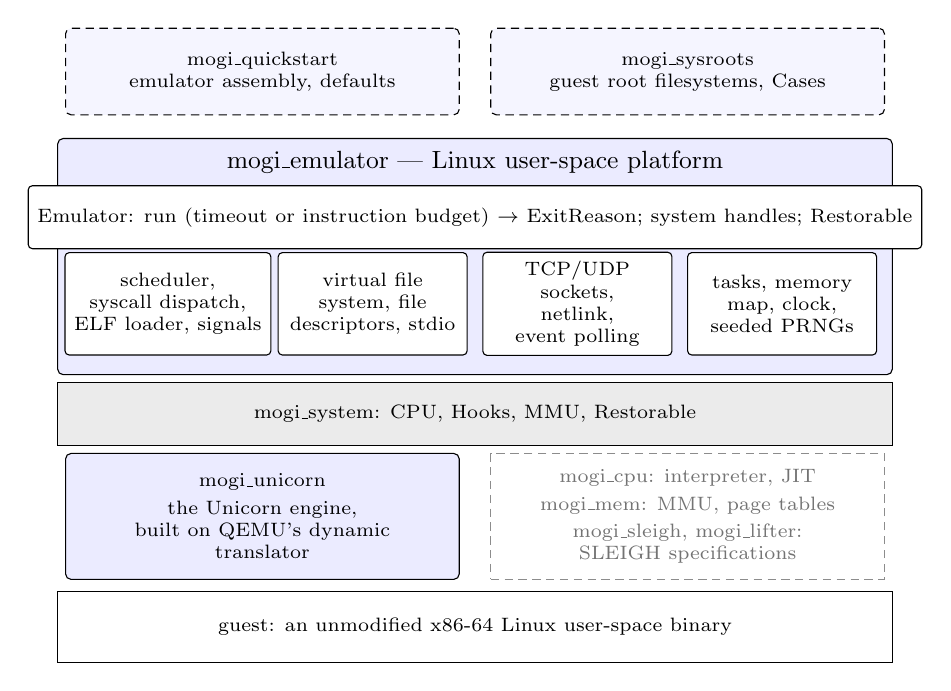
\begin{tikzpicture}[
      font=\small,
      layer/.style   = {draw, rounded corners=2pt, fill=blue!8, align=center},
      setup/.style   = {draw, rounded corners=2pt, densely dashed, fill=blue!4,
                        align=center, font=\scriptsize,
                        minimum width=50mm, minimum height=11mm},
      iface/.style   = {draw, rounded corners=1.5pt, fill=white, align=center,
                        font=\scriptsize, minimum width=100mm, minimum height=8mm},
      svc/.style     = {draw, rounded corners=1.5pt, fill=white, align=center,
                        font=\scriptsize, minimum width=24mm, minimum height=13mm},
      seam/.style    = {draw, fill=black!8, align=center, font=\scriptsize,
                        minimum width=106mm, minimum height=8mm},
      backend/.style = {draw, rounded corners=2pt, fill=blue!8, align=center,
                        font=\scriptsize, minimum width=50mm, minimum height=16mm},
      alt/.style     = {draw=black!45, densely dashed, fill=white, text=black!55,
                        align=center, font=\scriptsize,
                        minimum width=50mm, minimum height=16mm},
      guest/.style   = {draw, fill=white, align=center, font=\scriptsize,
                        minimum width=106mm, minimum height=9mm},
    ]
    % --- setup: runs once, before any guest instruction executes -------------
    \node[setup] (quick) at (-2.7,3.05) {\code{mogi\_quickstart}\\
                                         emulator assembly, defaults};
    \node[setup] (sysr)  at ( 2.7,3.05) {\code{mogi\_sysroots}\\
                                         guest root filesystems, \code{Case}s};

    % --- the emulator core ---------------------------------------------------
    \node[layer, minimum width=106mm, minimum height=30mm] (emu) at (0,0.7) {};
    \node[font=\small] at (0,1.9)
      {\code{mogi\_emulator} --- Linux user-space platform};
    \node[iface] (iface) at (0,1.2)
      {\code{Emulator}: \code{run} (timeout or instruction budget)
       $\to$ \code{ExitReason}; system handles; \code{Restorable}};
    \node[svc] (sched) at (-3.9,0.1) {scheduler,\\syscall dispatch,\\ELF loader,
                                      signals};
    \node[svc] (fs)    at (-1.3,0.1) {virtual file\\system, file\\descriptors,
                                      stdio};
    \node[svc] (net)   at ( 1.3,0.1) {TCP/UDP\\sockets,\\netlink,\\event polling};
    \node[svc] (misc)  at ( 3.9,0.1) {tasks, memory\\map, clock,\\seeded PRNGs};

    % --- the seam: everything above is written against these traits ----------
    \node[seam] (seam) at (0,-1.3)
      {\code{mogi\_system}: \code{CPU}, \code{Hooks}, \code{MMU}, \code{Restorable}};

    % --- two implementations of the seam -------------------------------------
    \node[backend] (uni) at (-2.7,-2.6) {\code{mogi\_unicorn}\\[2pt]
                                         the Unicorn engine,\\
                                         built on QEMU's dynamic\\
                                         translator};
    \node[alt]     (nat) at ( 2.7,-2.6) {\code{mogi\_cpu}: interpreter, JIT\\[2pt]
                                         \code{mogi\_mem}: MMU, page tables\\[2pt]
                                         \code{mogi\_sleigh}, \code{mogi\_lifter}:\\
                                         SLEIGH specifications};

    % --- the guest -----------------------------------------------------------
    \node[guest] (guest) at (0,-4.0)
      {guest: an unmodified x86-64 Linux user-space binary};
  \end{tikzpicture}
  \caption[The MOGI platform]{%
    The MOGI platform.
    \code{mogi\_emulator} models a Linux user-space system --- process
    scheduling, system calls, a virtual filesystem, sockets, and the clock and
    random sources a guest observes --- and exposes it as one \code{Emulator}
    that runs until a budget is exhausted or the guest blocks or exits.
    It is written entirely against the traits in \code{mogi\_system}, which is
    the seam that makes the execution backend interchangeable: the same guest
    model runs on the external Unicorn engine or on MOGI's own interpreter and
    JIT, which lift guest code from Ghidra SLEIGH processor specifications.
    All experiments in this thesis use the Unicorn backend
    (\cref{sec:platform-emulation}); the native stack (dashed) is the
    alternative implementation of the same traits.
    The setup crates (top) compose the guest root filesystem and assemble the
    emulator once, before any guest instruction executes.
  }
  \label{fig:platform-architecture}
\end{figure}


It is implemented as a Rust workspace with multiple crates.
The core execution environment abstractions live in \code{mogi\_system} and provide
\gls{cpu} and \gls{mmu} traits to support multiple backends.
It also includes \code{Hooks} and \code{Restorable} traits that allow installation
of hooks for collecting instrumentation information and taking snapshots of the system
state and then restoring them.
Unicorn\index{Unicorn} is a popular emulator based on QEMU~\cite{bellard_qemu_2005} and is
wrapped by \code{mogi\_unicorn}, which includes it as an execution backend.
A second backend tailored to MOGI is under development.
Its main components are implemented in \code{mogi\_cpu} as well as \code{mogi\_mem}.
It strives to be more flexible, more correct and faster than Unicorn.
Because not all features are fully implemented yet, we use the
\code{mogi\_unicorn} backend for this thesis.
Including the native MOGI backend is left as future work.

Since the main goal is to emulate Linux userspace binaries, we also include a full Linux
user-space emulation framework under \code{mogi\_emulator}.
It provides a generic model of system components such as clocks, file systems,
network stacks and standard I/O, as well as concrete implementations of these components.
It also includes an ELF loader and scheduler to allow execution of guest binaries.

Combining the backend provided by \code{mogi\_system} as well as the userspace
emulation framework provided by \code{mogi\_emulator} is done via the \code{Emulator}
trait.
It allows access to system components as well as execution of the guest binary with
a given run limit.
The program \emph{yields}\index{yield} control back to the caller whenever it encounters a stopping
error condition like a missing syscall implementation or an unsupported instruction and
whenever it requires an external input to continue.
To allow a user to quickly get an emulator up and running without having to manually
create every component, we provide \code{mogi\_quickstart}, a wrapper that creates
a full emulator instance with sensible defaults.

Guest binaries as well as guest base systems are provided via \code{mogi\_sysroots}.
This includes systems like ubuntu2510, as well as case binaries like open62541,
live555, or tinydtls.
Guest systems and test binaries are built using Dockerfiles during the regular Cargo
build process.
